\section{Theory}

One of the applications of sequential logic flip-flop circuits are counter circuits. 
A binary counter can count from $0$ to $2^n-1$, where n is the
total number of bits in the counter. They can be constructed using a series of flip-flops where each flip-flop represents one bit of information.

\noindent Based on the application of clock pulse, there are two types of counter circuits:

\begin{itemize}
    \item \textbf{Asynchronous Counters} or ripple counters where the flip flops do not receive the same clock pulse at the same time. Each flip flop is triggered by the output of the previous flip flop, and therefore there exists some propagation delay. 
    \item \textbf{Synchronous Counters} where all the flip flops receive the same clock pulse at the same time and their outputs change simultaneously. This will result in the no propagation delay between the flip flops.
\end{itemize}

\subsection*{Frequency Division}

A frequency divider can be constructed from J-K flip-flops by taking the output
of one cell to the clock input of the next. The J and K inputs of each flip-flop
are set to 1 to produce a toggle at each cycle of the clock input. For each two
toggles of the first cell, a toggle is produced in the second cell, so its
output is at half the frequency of the first. The output of the fourth cell is hence
1/16 the clock frequency. The same device is useful as a binary counter.

Hence the output at any point has an exact 50\% duty cycle. The final
output clock signal will have a frequency value equal to the input clock frequency
divided by the MOD number of the counter. Such circuits are known as \textit{divide-by-n} counters, where \textit{n} is the number of counter stages used.

\begin{figure}[H]
    \centering
    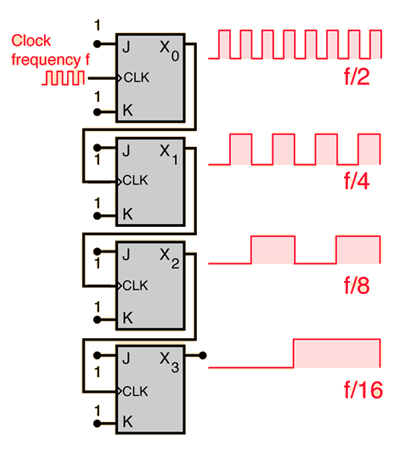
\includegraphics[width=0.6\columnwidth]{images/freqdiv2.png}
    \caption{An example of a frequency division circuit using JK flip flops}
    \label{fig:0}
\end{figure}

% ======================================================================================
\subsection{Binary Ripple Up Counter}
A 4-bit or MOD-16 ripple up counter can be constructed from 4 J-K flip-flops by taking the output of one cell to the clock input of the next. The J and K inputs of each flip-flop are set to 1 to produce a toggle at each cycle of the clock input. For each two toggles of the first cell, a toggle is produced in the second cell, so its output is at half the frequency of the first. The output of the fourth cell is 1/16 the clock frequency.

\begin{figure}[H]
    \centering
    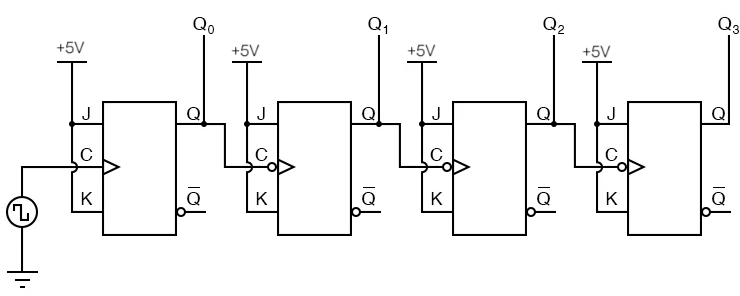
\includegraphics[width=1\columnwidth]{images/up2.png}
    \caption{Circuit diagram for a 4-bit binary ripple up counter. The PRESET and CLR pins are connected to HIGH}
    \label{up}
\end{figure}

The counting sequence corresponding to each input pulse is based on its binary representation in 4-bits (i.e. from 0000 to 1111). On supplying the 15th pulse the counter reads 1111 (decimal 15). The next clock
pulse after count 1111 will cause the counter to try to increment to 10000 (decimal 16).
However, that 1 bit is not held by any flip-flop and is therefore lost. As a result, the
counter actually reverts to 0000, and the count begins again.

\begin{figure}[H]
    \centering
    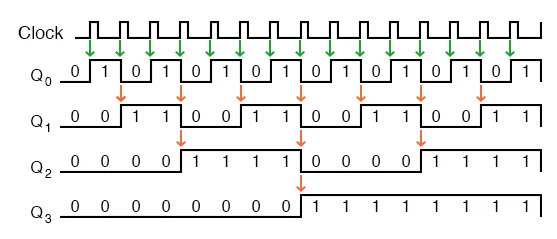
\includegraphics[width=1\columnwidth]{images/upplot.png}
    \caption{The ripple up circuit would yield the following output waveforms, when clocked by a repetitive source of pulses from a function generator}
    \label{upp}
\end{figure}
% ======================================================================================
\subsection{Binary Ripple Down Counter}

The binary ripple down-counter decreases the count by one each time a pulse
occurs at the input. Here, the complement
output of one flip-flop is connected to the clock input of the subsequent flip-flop. This toggles at each negative edge of the clock pulse (1 $\rightarrow$ 0 transition),
which is equivalent to a normal output toggling for the positive edge of the clock pulse (0 to
1 transition). Thus, the counter starts from 1111 with the first pulse after it is reset and reverts
back to 0000 on the 16th pulse.

\begin{figure}[H]
    \centering
    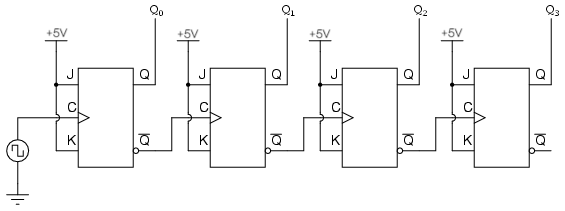
\includegraphics[width=1\columnwidth]{images/down.png}
    \caption{Circuit diagram for a 4-bit binary ripple down counter. The PRESET and CLR pins are connected to HIGH}
    \label{down}
\end{figure}
% ======================================================================================
\subsection{Modulus-N Counter}
The modulus of a counter is the number of discrete states a counter can take up. A
counter with $n$ no. of flip flops will have $2^n$ number of possible states. So counters with
modulus $2, 4, 8,\dots$ can be built up using $1, 2, 3, \dots$ flip flops. 

If one has to design a counter with $N$ states where $N$ is not a power of 2, we can construct a counter of the next higher power of 2, such that $2^n > N$ and then arrange the
circuit in such a way that it skips some of its natural states restricting it to $N$.

The simplest way of doing this is the \textit{direct clearing method}, where a gate circuit is used to
clear all the flip flops as the desired count is reached. For this an additional combinational logic circuit, a 4-input NAND gate is
required, whose output is connected to clear (\verb|CLR|) terminal of all the flip flops. This will feed a 
reset pulse to the counter during state $N$ so that immediately after state $N-1$.Hence, the flip-flops are reset and the counter starts counting again.

For example here is the circuit diagram for a MOD-12 counter. This will feed a reset pulse during state 12 (1100). So the counter will run from 0000 to 1011 and then loop back again to 0000 on the 12th pulse.

\begin{figure}[H]
    \centering
    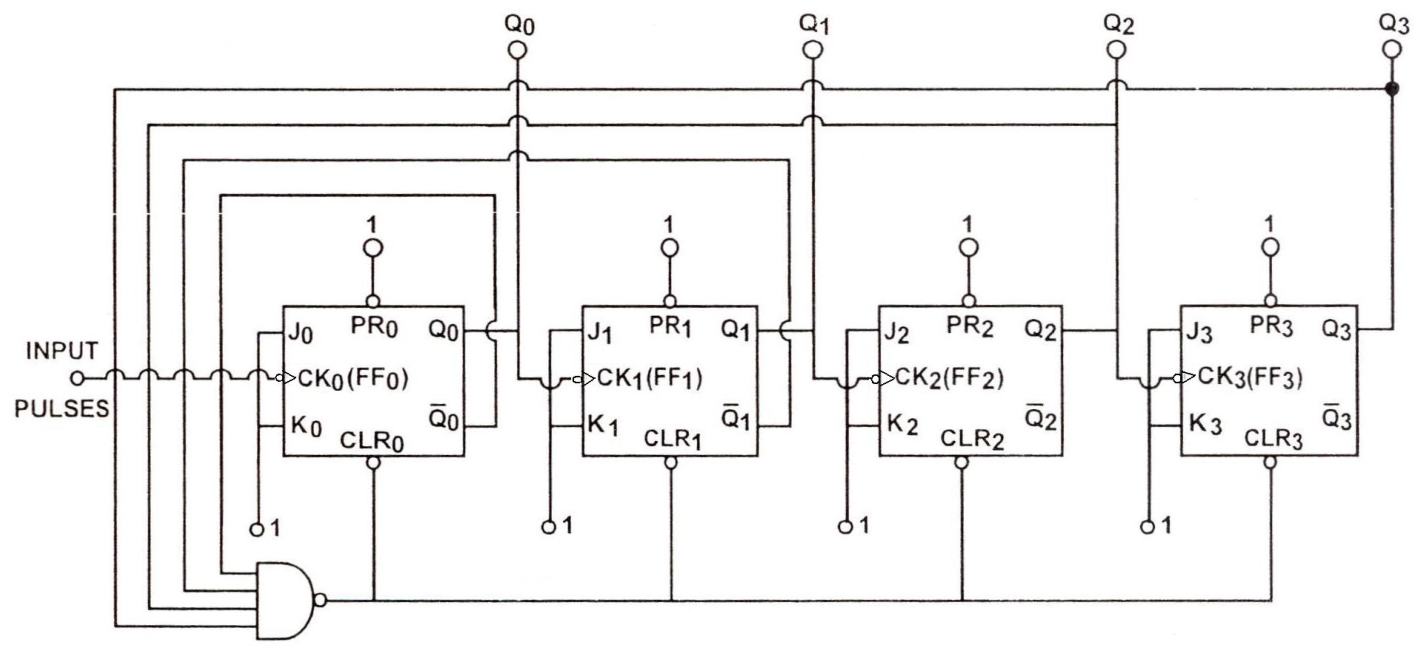
\includegraphics[width=1\columnwidth]{images/mod12.png}
    \caption{Circuit diagram for a MOD-12 ripple up counter}
    \label{mod}
\end{figure}
% 
% ======================================================================================
\subsection{Ring Counter}
A \textit{shift register} is a type of digital circuit using a cascade of flip-flops where the output of one flip-flop is connected to the input of the next. They share a single clock signal, which causes the data stored in the system to shift from one location to the next. A ring counter is a special type of Shift register where the output of the last flip flop is passed to the first flip flop as an input. This configuration creates a cyclic shift of the data bits through the flip-flops.

When a clock signal is applied to the ring counter, the data bits are shifted from one flip-flop to the next with each clock cycle. As a result, the ring counter generates a sequence of binary states that repeat after a specific number of clock cycles, depending on the number of flip-flops in the circuit. 

\begin{figure}[H]
    \centering
    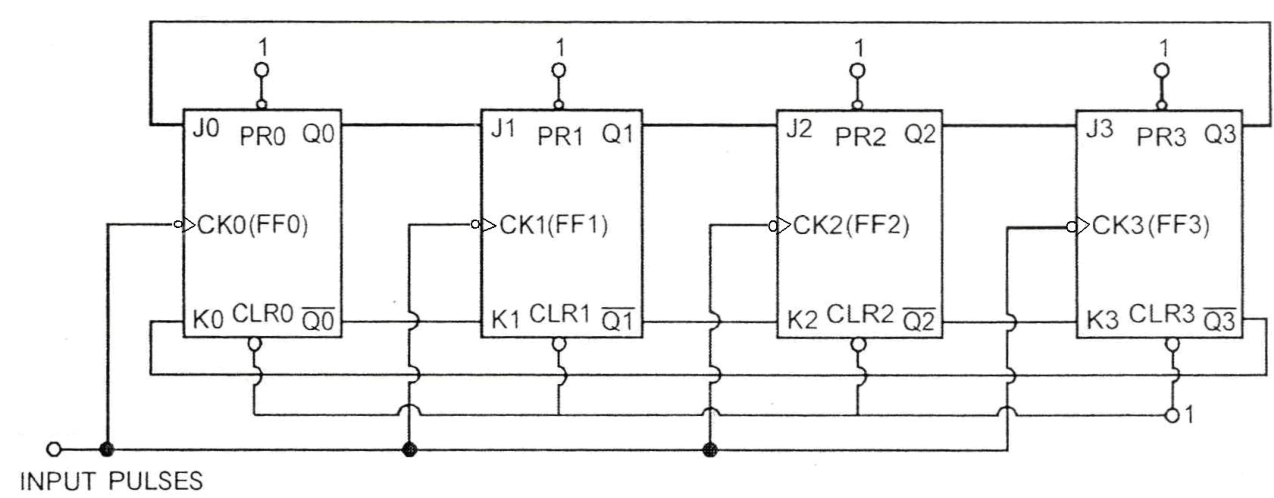
\includegraphics[width=1\columnwidth]{images/ring.png}
    \caption{Circuit diagram for a ring counter}
    \label{ring}
\end{figure}

\begin{figure}[H]
    \centering
    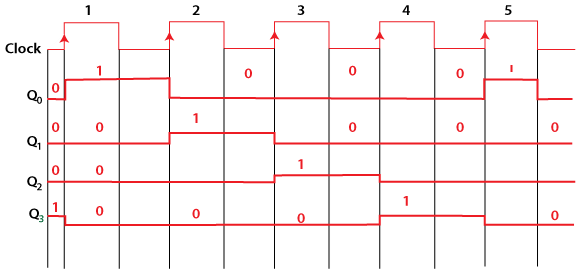
\includegraphics[width=1\columnwidth]{images/ring-counter5.png}
    \caption{Signal diagram for a ring counter circuit}
\end{figure}

Ring counter is extremely fast but it is uneconomical in the number of flip-flops.
This is overcome by a modified circuit known as a Johnson counter or switchtail ring
counter or twisted counter, where the outputs of the last flip-flop are crossed over and
then fed back to the first flip-flop. That is the normal and complement output of the last
flip-flop are connected to the K and J inputs of the first flip-flop respectively.

% ======================================================================================
\section{Experimental Setup}

\subsection*{Apparatus}

\begin{enumerate}
    \item ICs:
    \begin{enumerate}
        \item JK Flip-flop (FF-7476)
        \item 4-input NAND (7420)
    \end{enumerate}
    \item Resistors (1 k$\Omega$)
    \item DC Power Supply (5V)
    \item Function Generator
    \item Oscilloscope
    \item Breadboard
    \item Connecting Wires
\end{enumerate}

\subsection*{IC Pinout Diagrams}

\begin{figure}[H]
    \centering
    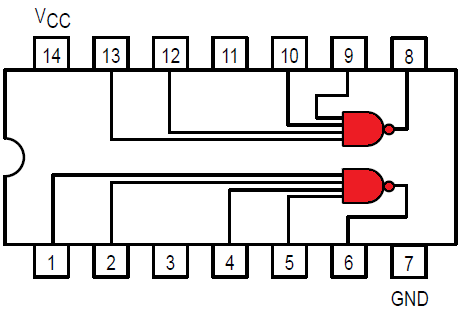
\includegraphics[width=0.6\columnwidth]{images/nand.png}
    \caption{IC pinout diagram for a 4 input NAND gate (IC 7420 )}
\end{figure}

\begin{figure}[H]
    \centering
    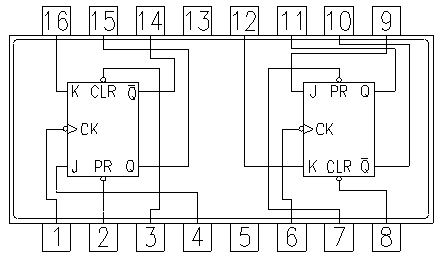
\includegraphics[width=0.75\columnwidth]{images/jk.png}
    \caption{IC pinout diagram for a JK flip flop (IC 7476)}
\end{figure}